\documentclass[12pt]{amsart}
\usepackage{geometry}                % See geometry.pdf to learn the layout options. There are lots.
\geometry{letterpaper}                   % ... or a4paper or a5paper or ... 
%\geometry{landscape}                % Activate for for rotated page geometry
\usepackage[parfill]{parskip}    % Activate to begin paragraphs with an empty line rather than an indent
\usepackage{graphicx}
\usepackage{amssymb}
\usepackage{epstopdf}
\usepackage{natbib}
\usepackage{hyperref}
\usepackage{url}
\usepackage{subfig}
\captionsetup[subfigure]{margin=0.5cm}
\captionsetup[subtable]{margin=0.5cm}
\DeclareGraphicsRule{.tif}{png}{.png}{`convert #1 `dirname #1`/`basename #1 .tif`.png}

\title{Modelling ecological communities as if they were DNA}
\author{William D. Pearse}
\date{\today}                                           % Activate to display a given date or no date
\begin{document}
\bibliographystyle{besjournals}
\maketitle
\section{Abstract}
Ecologists are interested in understanding and predicting how ecological communities change through time. While it might seem natural to measure this through changes in species' abundances, practical limitations often mean this is not possible. I present an approach inspired by DNA substitution models that attempts to estimate historic interactions between species, and from this attempts to estimate rates of turnover in ecological communities. As an example with simulated data shows, the method is not yet complete, but another example using UK butterfly community data shows the method may have promise. Areas of future work are also discussed.

\section{Introduction}
Ecologists tend to recognise broad habitat types and sub-types, grouping communities they define as similar in structure. A perfect example is the British National Vegetation Classification system \citep{Rodwell1991}, which hierarchically classifies all plant communities with the UK. However, ecologists also recognise a wide variety of variability within these categories, and the recent interest in Neutral Theory \citep{Hubbell2001} and stochastic variation at all spatial scales \citep{Vellend2010} suggests ecologists want to model this variation. However, models that allow for interspecific differences are often over-parameterised, and summary statistics of structure do not necessary help us make future predictions about species composition.

One way round this problem has been to model a community as proceeding through a series of states, each with their own associated species compositions and abundances. The probability of moving through between these states can be modelled using Markov Chains, and thus meaningful predictions can be made. This seems a natural way to model the habitat types that were discussed above, but ignores the continuous turnover within the states we are interested in, assumes the history of a community is unimportant, and requires that a system reaches a final, stable state \cite{Logofet2000}. Moreover, such methods require \emph{a priori} definitions of states, and as such cannot be driven by the data themselves.

My alternative is to model species turnover as a transition matrix, where the likelihood of a species entering a community can be predicted by the identity of the species they replace, creating a model with species-level parameters and predictions. The problem of over-parameterisation can be solved by simplification of this matrix, in much the way that a DNA or protein substitution matrix is often simplified by allowing certain bases or amino acids to share parameters. However, this method has the major drawback of requiring an accurate way of determining the history of species interactions in a community, when only observational data are actually available.

\section{Methods}
\subsection{Overview and Description of Problem}
I modelled the fate of each individual in a community over a number of discrete time-steps, and attempted to estimate parameters of interest for each species in a community based on what each individual did. I assumed an individual could do one of only three things in each time-step:
\begin{itemize}
\item Reproduction. That individual dies, and is replaced by another of the same species, or that individual survives to the next time-step.
\item Replacement. That individual dies, and is replaced by another of a different species.
\item Death. That individual dies, but is not replaced by another of any species.
\end{itemize}

Additionally, I allowed any number of individuals (of any number of species) to enter the community at each timestep. This allowed communities to increase in overall abundance through time.

This model makes no attempt to understand the processes driving any of these events; indeed, it is unclear whether a species `entering' the community has done so through immigration or an already-present member of the community having more than one offspring. A wide variety of different models were tried, but this model proved the quickest and most reliable to parameterise.

While this model is fairly simple, it is difficult to estimate the parameters involved (the rate of reproduction, loss, death and immigration) for each species because the history of the community is not clear from the identities of the species in a community. Taking table \ref{turnoverProblem} as an example, it is difficult to tell what happened between the first and second measurements of that community that led to species A increasing in number and species B become less abundant. Any attempt to infer what events were most likely to have happened requires an estimate of the relative likelihoods of those events taking place, creating a circularity.
\begin{table}
\centering
\subfloat[First Community]{
\begin{tabular}{l l}\hline
Species&Abundance\\ \hline
A&10\\
B&20\\
C&20\\ \hline
\end{tabular}}
\subfloat[Second Community]{
\begin{tabular}{l l}\hline
Species&Abundance\\ \hline
A&20\\
B&10\\
C&20\\ \hline
\end{tabular}}
\caption{The problem of estimating species turnover. What happened in the time between the first measurement of this community (A) and the second (B)? Did ten individuals of species B become replaced by ten of species A? Did ten individuals of species B die out without leaving descendants, and ten members of species A come from outside the community? Did ten individuals of species C become replaced by ten of species A, and another ten came in from outside the community? There are an almost infinite number of possible transitions between the two communities, and no obvious way to determining the best route without already having a model of the likelihood of all the possible transitions.}
\label{turnoverProblem}
\end{table}
\subsection{Description of Method}
The method assumes the community composition of a certain number of communities, each with a number of repeated measurements taken at the same, regular time intervals, are perfectly known. It then generates a null \emph{transition matrix} (table \ref{transMatEg}), which contains the relative rates of reproduction, replacement, death, and addition (defined above) for each species. Note that within each row all bar the last column must sum to one (since each individual must do \emph{something} in each time step), while in the last column all the rows must sum to one since every time an individual enters the community it must be of \emph{a} species.
\begin{table}
\begin{center}
\begin{tabular}{c|cccc|c}
&A&B&C&Death&Addition\\ \hline
A&reproduction&replacement&replacement&death&addition\\
B&replacement&reproduction&replacement&death&addition\\
C&reproduction&replacement&replacement&death&addition\\
\end{tabular}\\
\caption{Example \emph{transition matrix}. Each species is a represented by letter (`A', `B', and `C'), and each element represents a parameter of the model, as described in \textsection3.1.}\label{transMatEg}
\end{center}
\end{table}

Then, at random, each individual recorded in a community at a given time has its most likely source (be it a reproduction, replacement or addition from any particular species) calculated given the number of individuals in that community's previous time step that haven't already been assigning to another event. If a community has fewer individuals than the previous time step, the most likely species to have died is calculated and an individual of that species assigned to that event in much the same way. This creates an \emph{event matrix} , of the same dimensions as the \emph{transition matrix}, with counts of the number of times each possible event in the \emph{transition matrix} took place.

Each parameter in the \emph{transition matrix} (in a random order) is estimated using Brent's method, each time re-calculating the \emph{event matrix}  and scaling the other parameters so that in each row all elements bar the last sums to one, and in the last column all the elements sum to one. This process of recalculating the entire \emph{transition matrix} can be iterated as many times as is required, and while at present only one null matrix can be used as a starting position there is no reason more matrices couldn't be used as starting points.

The program is written in C++, making use of the BOOST library. This document, and all its code, is available online at \href{http://www.github.com/willpearse/lottery}{\url{http://www.github.com/willpearse/lottery}}.
\section{Example with Simulated Data}
It is possible to run the program with a single command-line option (a random seed) that causes it to generate ten random communities, each with ten years of data, starting with 100 individuals and having ten individuals added at each time-step. The program then performs one search, with five iterations, and returns the estimated matrices. I present an example of running the code like this, with the random seed `123456'. Tables \ref{simTrans} and \ref{simEvent} show the simulated and estimated \emph{transition} and \emph{event} matrices, along with the null \emph{transition matrix} used to start the search.

It is clear that the method has not performed perfectly. Although species with higher reproduction rates have higher estimated rates, the estimates are inflated, the method is poor at detecting death events, and underestimates rates of addition. I think these problems reflect the fact that all transition and death rates for a species are identical, as are all species' addition rates. There likely exist a number of equally-likely ways of explaining these results, and I feel the model has got caught in a local optimum, something that repeated searches from different locations might help detect. In particular, note that the death parameter for most species is quite close to 0.1 --- given there are ten additions at each time step, and the communities start with 100 individuals, the rates of death and immigration are so close for most species it may be difficult for the program to detect what is going on. Indeed, note that the species with the lowest rate of death (`c') also has the highest estimated addition rate.
\begin{table}
\centering
\subfloat[Real]{
\begin{tabular}{l |llllll |l}
&a&b&c&d&e&Death&Addition\\ \hline
a&{\bf0.46}&0.11&0.11&0.11&0.11&0.11&0.20\\
b&0.07&{\bf0.66}&0.07&0.07&0.07&0.07&0.20\\
c&0.02&0.02&{\bf0.88}&0.02&0.02&0.02&0.20\\
d&0.03&0.03&0.03&{\bf0.85}&0.03&0.03&0.20\\
e&0.09&0.09&0.09&0.09&{\bf0.53}&0.09&0.20\\
\end{tabular}}\\
\subfloat[Null]{
\begin{tabular}{l |llllll |l}
&a&b&c&d&e&Death&Addition\\ \hline
a&{\bf0.20}&0.16&0.16&0.16&0.16&0.16&0.20\\
b&0.16&{\bf0.20}&0.16&0.16&0.16&0.16&0.20\\
c&0.16&0.16&{\bf0.20}&0.16&0.16&0.16&0.20\\
d&0.16&0.16&0.16&{\bf0.20}&0.16&0.16&0.20\\
e&0.16&0.16&0.16&0.16&{\bf0.20}&0.16&0.20\\
\end{tabular}}\\
\subfloat[Estimated]{
\begin{tabular}{l |llllll |l}
&a&b&c&d&e&Death&Addition\\ \hline
a&{\bf0.65}&0.01&0.12&0.11&0.02&0.01&0.23\\
b&0.03&{\bf0.84}&0.06&0.05&0.01&0.01&0.16\\
c&0.00&0.01&{\bf0.96}&0.01&0.00&0.01&0.2771\\
d&0.01&0.01&0.01&{\bf0.95}&0.01&0.01&0.01\\
e&0.01&0.06&0.04&0.052&{\bf0.82}&0.01&0.32\\
\end{tabular}}
\caption{Values of the \emph{transition matrix} used to generate the data (A), as the null to start the search procedure (B), and given as the estimated result (C). The diagonal elements have been highlighted. This example shows a general tendency of the program to under-estimate death, and to over-estimate the likelihood of an individual to reproduce.}\label{simTrans}
\end{table}
\begin{table}
\centering
\subfloat[Real]{
\begin{tabular}{l |llllll |l}
&a&b&c&d&e&Death&Addition\\ \hline
a&{\bf566}&121&148&150&131&136&169\\
b&125&{\bf1234}&123&111&124&122&195\\
c&88&92&{\bf2785}&79&80&63&173\\
d&108&93&92&{\bf2447}&82&85&166\\
e&126&130&137&143&{\bf786}&120&197\\
\end{tabular}}\\
\subfloat[Estimated]{
\begin{tabular}{l |llllll |l}
&a&b&c&d&e&Death&Addition\\ \hline
a&{\bf896}&12&96&93&57&8&45\\
b&84&{\bf1627}&78&24&26&0&63\\
c&11&34&{\bf3104}&27&10&1&116\\
d&22&28&33&{\bf2785}&38&1&106\\
e&34&101&31&61&{\bf1215}&0&54\\
\end{tabular}}
\caption{Values of the \emph{event matrix} used to generate the data (A), and estimated at the end of the run (B). The diagonal elements have been highlighted. This example shows a general tendency of the program to under-estimate death, and to over-estimate the likelihood of an individual to reproduce.}\label{simEvent}
\end{table}
\section{Example with Ecological Data}
Butterfly community data were taken from the UK Butterfly Monitoring Scheme (UKBMS), a scheme that has repeatedly-sampled butterfly community data dating back to 1974. A phylogeny of all the species in the dataset (figure \ref{phylogeny}) was generated using the cytochrome oxidase one gene and BEAST \citep{Drummond2006,Drummond2007,Drummond2012}, fitting constraints at the family level to keep the phylogeny in line with previous studies \citep{Mutanen2010,Wahlberg2010}.
\begin{figure}
\begin{center}
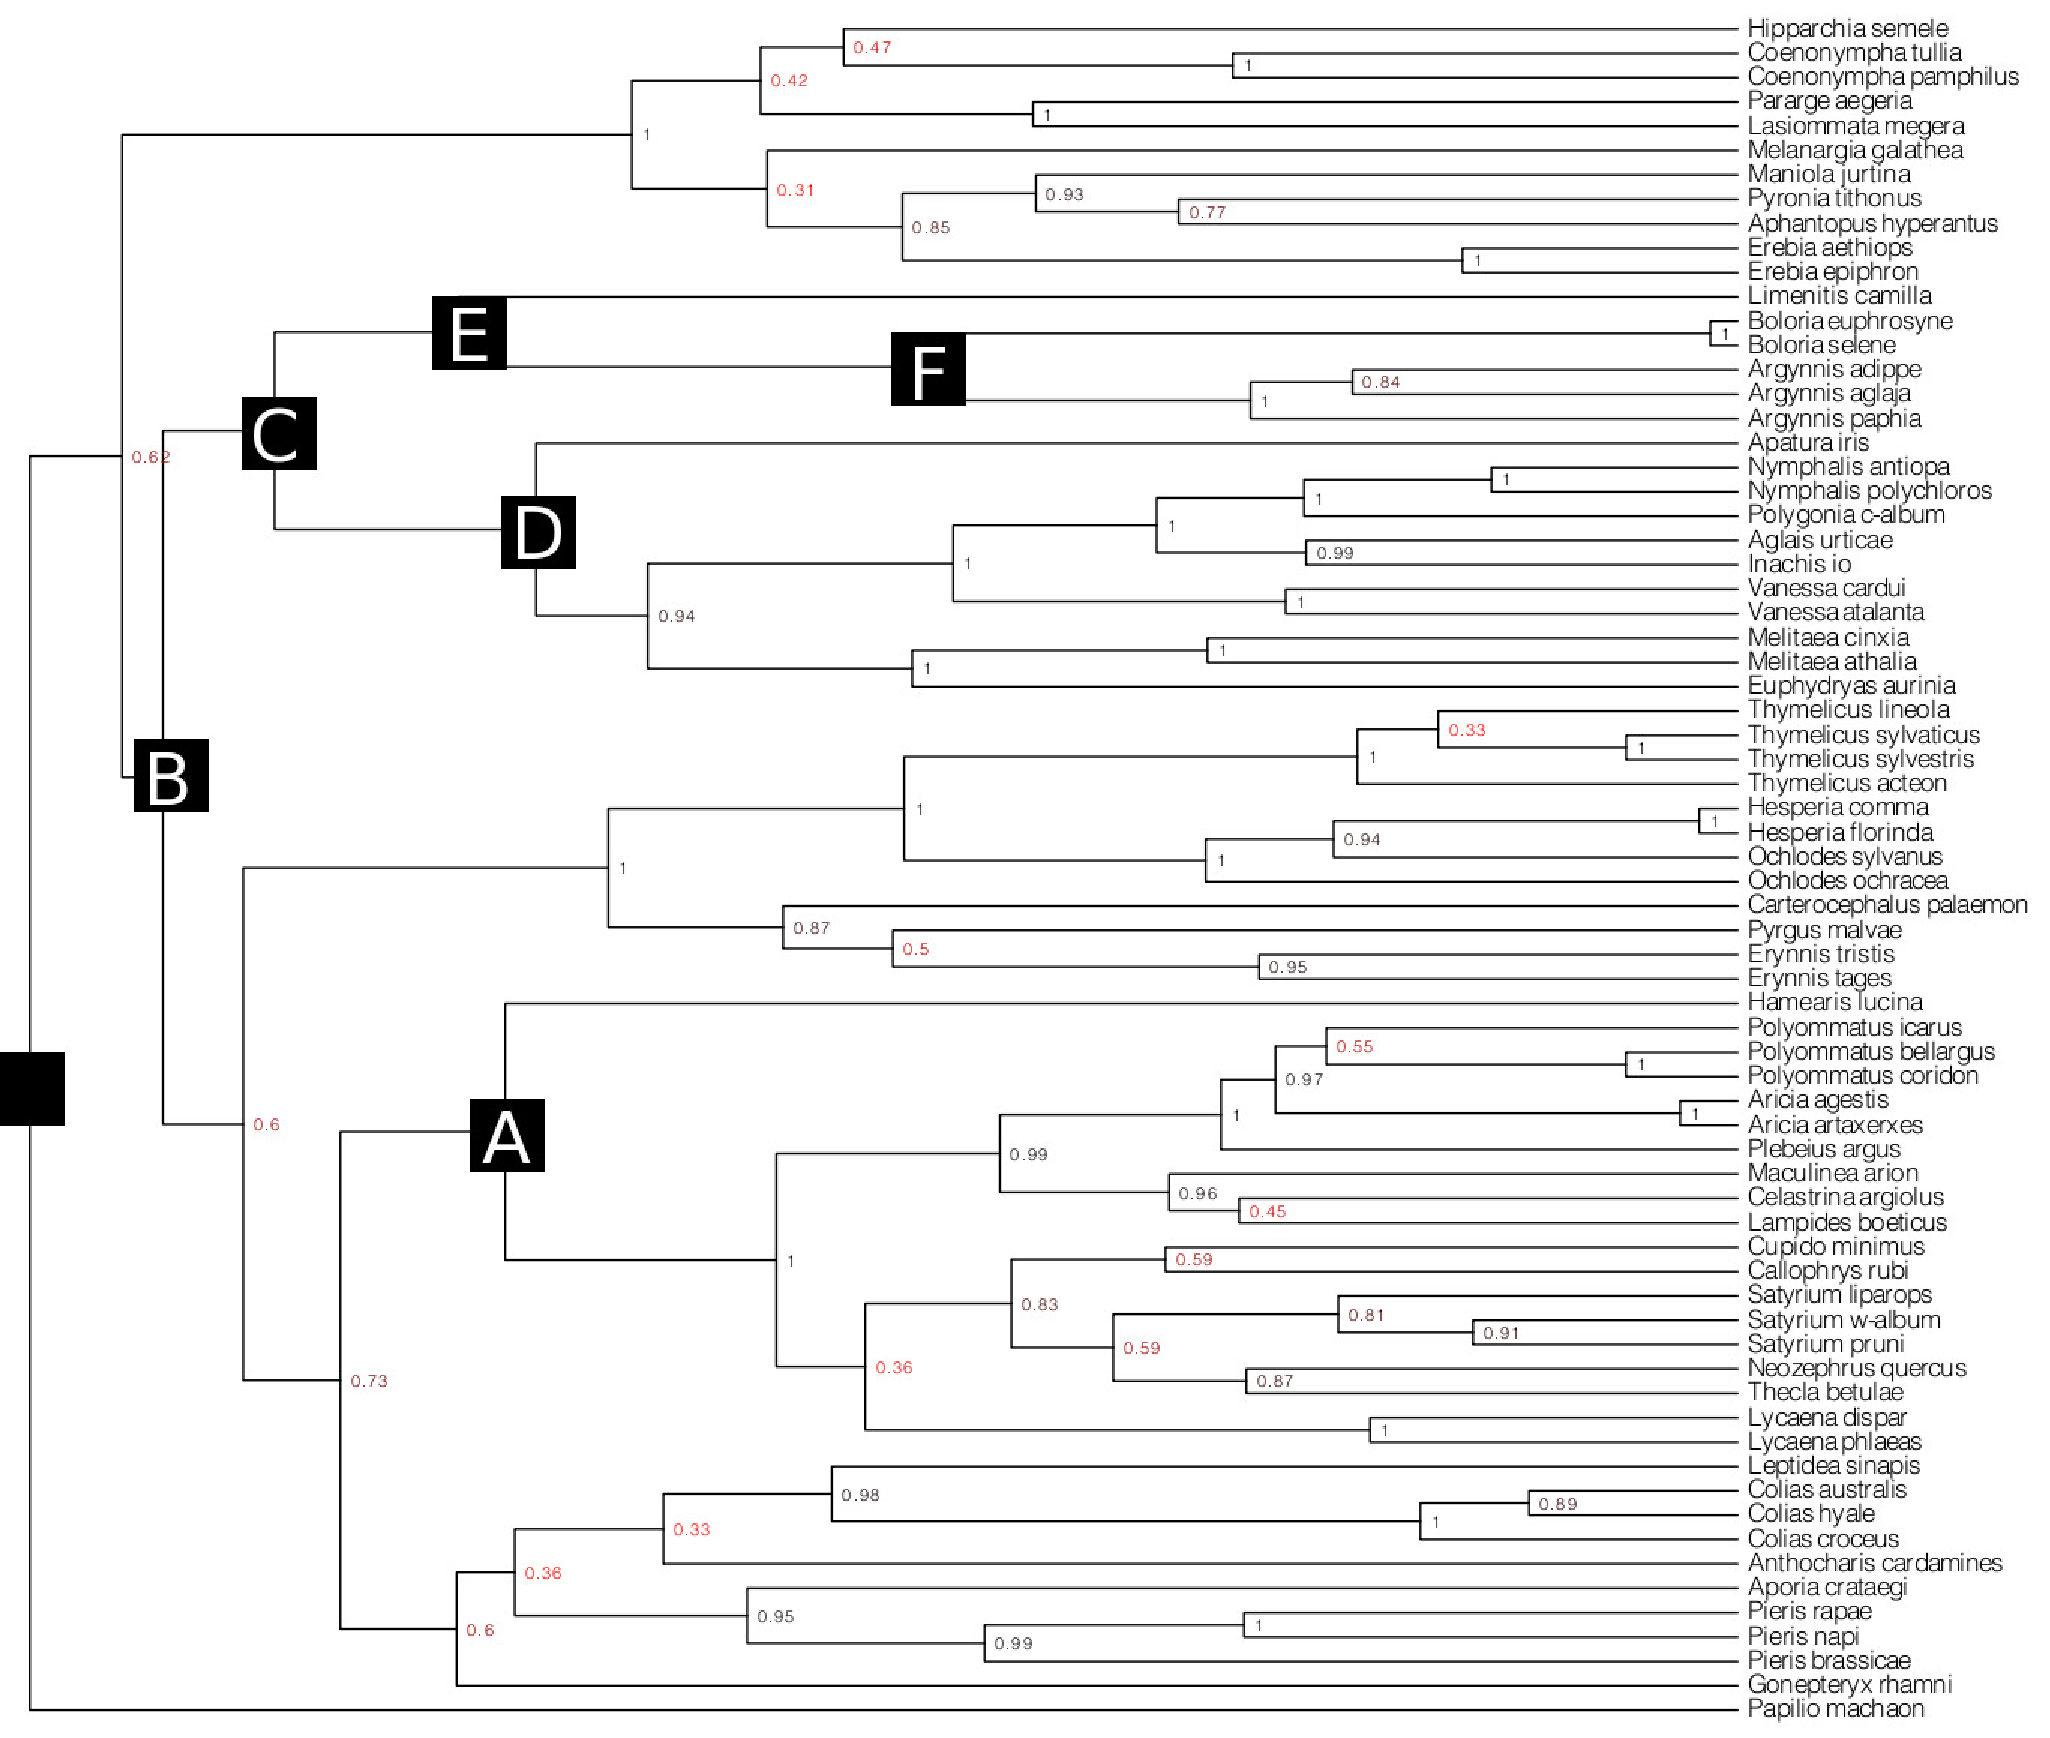
\includegraphics[width=\textwidth]{phylogeny}
\caption{Butterfly phylogeny. Letters at clades are the identifiers given to each clade used in the analysis. Numbers at nodes indicate posterior probabilities; the more read a number, the less support there is for that node. Note that \emph{Papilio machaon}, which is at the root, was excluded from the analysis. More complete details of the construction of the phylogeny are available from the author on request.}
\label{phylogeny}
\end{center}
\end{figure}

The best-recorded site's yearly species abundances were split into five clades (marked on the figure \ref{phylogeny}), and the abundances in each clade used as input for the program. While grouping the butterflies in this way may seem unusual, it reduces the complexity of the problem, and is reasonable in a system where ecological traits are known to be highly conserved, and where I have shown strong phylogenetic patterns to the data in previous work. The results, after only one search with five iterations, are shown in table \ref{ecolResults}. I do not have permission to distribute the butterfly data, and so the input file cannot be included in the release of this code.
\begin{figure}
\centering
\subfloat[\emph{Transition Matrix}]{
\begin{tabular}{l |llllll |l}
&A&B&C&D&E&Death&Addition\\ \hline
A&{\bf0.38}&0.01&0.02&0.01&0.01&0.57&0.04\\
B&0.30&{\bf0.22}&0.04&0.01&0.07&0.35&0.03\\
C&0.00&0.00&{\bf0.99}&0.00&0.00&0.00&0.01\\
D&0.15&0.01&0.08&{\bf0.15}&0.15&0.45&0.68\\
E&0.01&0.00&0.01&0.00&{\bf0.95}&0.01&0.24\\
\end{tabular}}\\
\subfloat[\emph{Event Matrix}]{
\begin{tabular}{l |llllll |l}
&A&B&C&D&E&Death&Addition\\ \hline
A&{\bf16016}&590&76&64&1052&3556&2408\\
B&497&{\bf2208}&237&153&481&119&443\\
C&380&61&{\bf863}&6&188&107&242\\
D&168&30&71&{\bf358}&73&40&78\\
E&2039&386&83&98&{\bf6495}&930&1759\\
\end{tabular}}\\
\caption{Values of the \emph{transition} and \emph{event} matrices when the method was applied to real data. See text for further discussion, but note that these parameters do not resemble those of the simulated data, in particular having large `death' parameter estimates.}\label{ecolResults}
\end{figure}

Clearly it is not appropriate to make strong claims about the validity of these results, but a general point can be made. These matrices are much more variable in terms of parameters that those estimated from the simulated data. This suggests that, even though the fitting process is unlikely to have yet been perfected, there appears to be some signal in this data, probably reflecting the biology of the system. Few of the clades seem to be interacting with other clades, in that their replacement parameters are often quite low. An interesting exception to this is species `B', which has an asymmetrical interaction with species `A'.
\section{Further Work}
I have chosen a simulated example that shows the problems remaining with the method, and it makes it clear that the method may need more to work to fix some remaining issues. Once this has been done, some more rigorous sets of analyses, setting the method against different kinds of simulated data, will be necessary to demonstrate that the method can work in ideal conditions. My feeling is that butterfly data may still be a good test case for its use with real data, because many butterflies have non-overlapping generations and cannot over-winter, fitting some of the assumptions of the model.

At present, an over-parameterised model is fit to the data. This clearly is not appropriate, but simplification of the \emph{transition matrix} has not been too difficult in some tests I have run. Stepwise addition of model parameters, starting with a null matrix and adding a species-specific parameter wherever the likelihood of the model is increased the most, is entirely possible but can take a long time. However, there are still ways in which the program can be sped up, particularly by reducing its dependency on the BOOST matrices, and it is unlikely that the \emph{event matrix} needs to be recalculated each iteration through Brent's method. Thus a stepwise addition method, combined with a slightly faster execution, may be the way forward. It would be useful to see if the parameters of these matrices change over time, to identify tipping-points in the ecology of a system. Finding such a threshold would not be difficult with time series data such as these, as partitions should clearly be continuous in time and so for a dataset with ten years there could only be nine possible partitions.
\section{Acknowledgements}
I am grateful to the Heidelberg Institute for Theoretical Studies for funding my time in Heidelberg, which I enjoyed very much. I spent a wonderful three months with Alexei, Andre, Christian, Fernando, Kassian, Jiajie, Pavlos and Solon, and I'm hopeful that they won't laugh too much while reading through this on a Thursday night.

\bibliography{Library}
\end{document}  